% Propietario conservado: /Users/ruben/Documents/New project/output/REVISION_ARGUMENTAL_APERTURAS_CIERRES_20260915/VIII/spanish_source/ampliacion/centro_frontera.tex
\section{Centro, frontera y vacancias en la conexión nonádica}
\label{viii:sec:centro-frontera}
\subsection{La tesis y el orden de construcción}
La relación entre centro y frontera adquiere contenido matemático cuando se precisa qué datos se publican, qué transformaciones los transportan y con qué información se reconstruyen. En APP, un residuo se acompaña de su cociente; en TRIT, la orientación distingue operaciones que un agregado puede reunir; en TPK, una vuelta devuelve la fase y prolonga la memoria. El estado enriquecido reúne esas coordenadas. Su residencia en la estructura discreta conjunta del continuo conserva las dependencias entre las distintas lecturas posteriores.

El recorrido es APP → TRIT → TPK → estado enriquecido → estructura discreta conjunta del continuo. Este desarrollo efectúa cortes locales de ese recorrido: no reconstruye los cinco aspectos consustanciales del continuo desde una forma espectral ni los transforma en cinco módulos independientes. Las constantes internas se reciben en su etapa de publicación, sin utilizar sus valores convencionales para elegir semillas, rutas o coeficientes.

La intuición autoral puede expresarse así: \textbf{la publicación de un valor es una proyección de una construcción; para transportar esa construcción se conserva la información que permite distinguir sus realizaciones}. Las operaciones siguientes concretan esa afirmación. El lenguaje posterior de interpolación y de descomposición ortogonal demuestra propiedades de objetos ya especificados; no selecciona retrospectivamente el estado APP.

\subsection{La corona local y la reconstrucción del centro}
En la carta positiva se utiliza

\[
\rho_9(n)=1+[(n-1)]_9,\qquad
q_9(n)=\frac{n-\rho_9(n)}9,
\qquad n=\rho_9(n)+9q_9(n).
\]
La tabla producto es \(P(i,j)=ij\), con \(1\leq i,j\leq9\). La restricción a \(Q=\{3,4,5,6\}^2\) publica

\[
\left(\rho_9(ij)\right)_{i,j=3}^{6}=
\begin{pmatrix}
9&3&6&9\\
3&7&2&6\\
6&2&7&3\\
9&6&3&9
\end{pmatrix}.
\]

% BEGIN OWNER /Users/ruben/Documents/New project/output/REVISION_ARGUMENTAL_APERTURAS_CIERRES_20260915/VIII/spanish_source/ampliacion/figura_centro_frontera.tex
\begin{figure}[htbp]
\centering
\begin{minipage}[c]{.46\textwidth}
\centering
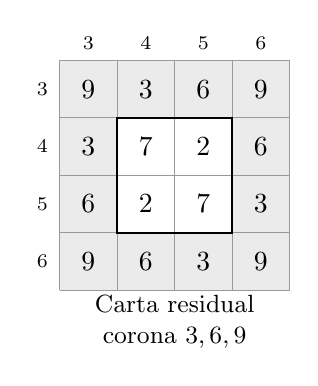
\begin{tikzpicture}[x=.73cm,y=.73cm]
\fill[black!8] (0,0) rectangle (4,4);
\fill[white] (1,1) rectangle (3,3);
\draw[step=1,black!40] (0,0) grid (4,4);
\draw[thick] (1,1) rectangle (3,3);
\foreach \row/\vals in {0/{9,3,6,9},1/{3,7,2,6},2/{6,2,7,3},3/{9,6,3,9}}{
  \foreach \val [count=\col from 0] in \vals{
    \node at (\col+.5,3.5-\row) {\(\val\)};
  }
}
\foreach \v [count=\n from 0] in {3,4,5,6}{
  \node[font=\scriptsize] at (\n+.5,4.3) {\(\v\)};
  \node[font=\scriptsize] at (-.3,3.5-\n) {\(\v\)};
}
\node[font=\small,align=center] at (2,-.55) {Carta residual\\corona \(3,6,9\)};
\end{tikzpicture}
\end{minipage}\hfill
\begin{minipage}[c]{.50\textwidth}
\centering
\begin{tikzpicture}[x=.73cm,y=.73cm]
\fill[black!3] (0,0) rectangle (4,4);
\draw[black!40] (0,0) rectangle (4,4);
\draw[thick] (1,1) rectangle (3,3);
\foreach \x/\y/\v in {.5/3.5/9,3.5/3.5/18,.5/.5/18,3.5/.5/36,
  1.5/2.5/16,2.5/2.5/20,1.5/1.5/20,2.5/1.5/25}{
  \node at (\x,\y) {\(\v\)};
}
\draw[-{Stealth},black!60] (.85,3.15) -- (1.22,2.78);
\draw[-{Stealth},black!60] (3.15,3.15) -- (2.78,2.78);
\draw[-{Stealth},black!60] (.85,.85) -- (1.22,1.22);
\draw[-{Stealth},black!60] (3.15,.85) -- (2.78,1.22);
\node[font=\small,align=center] at (2,-.55) {Frontera levantada\\e interpolación multiafín};
\end{tikzpicture}
\end{minipage}
\caption{La misma carta en dos lecturas. A la izquierda, la corona radical rodea el bloque \(B_c\). A la derecha, las cuatro esquinas enteras determinan los valores interiores bajo la ley multiafín. Sus residuos de esquina coinciden, pero los cocientes \((0,1,1,3)\) distinguen el levantamiento.}
\label{viii:fig:centro-frontera}
\end{figure}

% END OWNER


\Needspace{6\baselineskip}
Su bloque interior es

\[
B_c=\begin{pmatrix}7&2\\2&7\end{pmatrix}.
\]
El perímetro de esta carta contiene doce posiciones: cuatro con valor \(3\), cuatro con \(6\) y cuatro con \(9\); su suma es \(72\). Se hace visible una corona radical alrededor del bloque central. El centro electrónico global es \((5,5)\), único punto fijo de la inversión de la APP completa; no se cambia su posición al elegir esta carta local, cuyo centro geométrico está en \((4.5,4.5)\).

\begin{proposition}[Recuperación desde la frontera levantada]
\label{viii:prop:centro-frontera-recuperacion}
Sea \(F(x,y)=a+bx+cy+dxy\) una ley multiafín en la carta \([3,6]^2\). Para \(t=(x-3)/3\) y \(u=(y-3)/3\),

\[
\begin{aligned}
F(x,y)={}&(1-t)(1-u)F(3,3)+(1-t)uF(3,6)\\
&+t(1-u)F(6,3)+tuF(6,6).
\end{aligned}
\]
\end{proposition}
\begin{proof}
Para \(y\) fijo, la afinidad en \(x\) recupera \(F(x,y)\) desde \(F(3,y)\) y \(F(6,y)\). La afinidad en \(y\) recupera cada uno de esos dos valores desde sus extremos. La composición da la fórmula. En particular, las cuatro esquinas determinan toda la carta dentro del espacio de leyes declarado.
\end{proof}

Para el producto, los cuatro valores levantados son \(9,18,18,36\). Sus residuos positivos son todos \(9\), pero sus cocientes son \(0,1,1,3\). La fórmula recupera \(16,20,20,25\) en las posiciones interiores; su publicación residual da \(7,2,2,7\). De este modo, la frontera determina el interior \textbf{conservando la ley y el levantamiento}. La interpolación se hace antes de la reducción modular: no se divide por \(3\) en \(\mathbb Z/9\mathbb Z\), donde \(3\) no es invertible.

Esto precisa el sentido de «conservar la información del centro». La corona residual por sí sola no individualiza todos los levantamientos: \(F\) y \(F+9\) tienen los mismos residuos en toda la frontera y distintos valores levantados. La pareja residuo–cociente elimina esa ambigüedad dentro de la reconstrucción indicada. La afirmación queda probada para las leyes multiafines; extenderla a estados completos requiere conservar también los operadores, las rutas y la memoria que actúan sobre ellos.

La recuperación multiafín es una \textbf{formalización nueva de la arquitectura autoral preexistente}. Las cartas y sus lecturas son resultados recuperados del corpus; esta presentación explícita de su inversa no se atribuye como un descubrimiento histórico independiente.

\subsection{Suma, producto y los tres valores de la curvatura discreta}
Las filas multiplicativas se construyen por acumulación aditiva. La diferencia entre ambas hojas aparece al variar simultáneamente las dos coordenadas. Con diferencias unitarias,

\[
\Delta_x\Delta_y(x+y)=0,
\qquad
\Delta_x\Delta_y(xy)=1.
\]
La misma propiedad se recupera en la frontera levantada:

\[
\frac{P(6,6)-P(6,3)-P(3,6)+P(3,3)}{3\cdot3}=1;
\]
para \(S(x,y)=x+y\), ese cociente vale \(0\). El producto registra la variación cruzada que la suma no introduce. El corpus expresa la versión orientada mediante

\[
\mathcal F(T_x,T_y)=\Delta_x\Delta_yT_y-\Delta_y\Delta_xT_x,
\]
\[
\mathcal F(S,S)=\mathcal F(P,P)=0,
\qquad \mathcal F(S,P)=+1,
\qquad \mathcal F(P,S)=-1.
\]
El orden de las hojas distingue el signo. La formulación «la suma acumula y el producto pliega o despliega» se apoya aquí en una operación verificable: al proyectar modularmente se conserva un residuo; al levantar se recupera el cociente que registra lo sobrepasado. La curvatura discreta registra además el orden de las variaciones. No se identifica esta diferencia finita con una curvatura diferencial de un espacio físico sin su mapa de realización correspondiente.

\subsubsection*{La cruz radical global}
En \(R=\mathbb Z/9\mathbb Z\), el ideal \(\mathfrak m=\{0,3,6\}\) satisface \(\mathfrak m^2=0\). Su publicación positiva es \(\{9,3,6\}\). La cruz

\[
(\mathfrak m\times R)\cup(R\times\mathfrak m)
\]
tiene \(27+27-9=45\) posiciones. La intersección contiene nueve valores \(9\), de suma \(81\); los brazos restantes tienen doce valores de cada clase \(3,6,9\), de suma \(216\). El total es

\[
297=216+81=3(72+27)=3\cdot99.
\]
Se distinguen cuatro fronteras: el perímetro local de doce posiciones, la cruz radical de cuarenta y cinco, el gnomon de diecisiete que completa \(8^2\) a \(9^2\), y la corona cúbica de \(271\). Cada una tiene dominio y operación propios. El cociente trítico \(R/\mathfrak m\) conserva una clase; transportar el estado requiere acompañarla de los datos levantados y de su historia.

\subsection{Los lectores 72–27, 77–22 y la completación 729–271}
Las filas ordenadas de \(B_c\) se publican decimalmente como \(72\) y \(27\); sus diagonales como \(77\) y \(22\). Resulta

\[
72+27=77+22=99.
\]
En la completación cúbica, el conteo de interior, caras, aristas y vértice da

\[
1000=729+243+27+1=729+271,
\]
\[
999=729+243+27=729+270.
\]
La coincidencia de lectores se expresa conservando el resto decimal:

\[
729=10\cdot72+9,\qquad271=10\cdot27+1.
\]
Por tanto, la lectura bidimensional publica \((72,27)\); la lectura cúbica publica \(((72,9),(27,1))\). La pareja de restos \((9,1)\) distingue las prolongaciones que compartirían un mismo cociente. Primero se efectúan las construcciones de las cartas; después se comparan esas publicaciones. La identidad de los enteros no invierte ese orden causal.

El capítulo de canales enteros proporciona otra composición específica. Con los recuentos internos \(\Delta=54\), \(\nu=\Delta/2=27\) y \(\Theta=5\nu=135\), obtiene

\[
\mathcal C_\alpha=\nu^2=729,
\qquad \mathcal C_e=2\Theta+1=271.
\]
Aquí se ha renombrado como \(\nu\) el entero local que ese propietario escribe \(\kappa\), para distinguirlo de la lectura racional del registro dodecafásico. Los canales son objetos enteros; su identificación con las constantes pasa por los lectores regionales y el cierre correspondiente, no por los primeros dígitos de una expansión. Esta comparación utiliza los canales enteros y no necesita la realización angular posterior.

Para la referencia oral a una fracción de \(\pi\), el propietario localizado contiene

\[
\frac{396}{126}=\frac{22}{7},\qquad
396=18+72+108+198,\quad126=18+108.
\]
Es una razón racional de anillos alternos. Esta razón de anillos es una lectura racional exacta; su función se distingue de la publicación regional de \(\pi\).

\subsection{El centro electrónico y sus vacancias conjugadas}
La inversión de la APP positiva es \(\rho(r,c)=(10-r,10-c)\). Su único punto fijo es \((5,5)\). En la fibra aditiva central,

\[
\mathcal F_{10}=\{(5+t,5-t):t\in\mathbb Z,\ |t|\leq4\},
\]
el producto vale \(25-t^2\). Conservar su residuo central exige \(t^2\equiv0\pmod9\), equivalente a \(3\mid t\). Los únicos lugares son, por tanto,

\[
(5,5),\qquad(8,2),\qquad(2,8).
\]
Si \(\mathcal A\) conserva la pareja residuo–cociente en cada hoja,

\[
\begin{aligned}
\mathcal A(5,5)&=((1,1),(7,2)),\\
\mathcal A(8,2)=\mathcal A(2,8)&=((1,1),(7,1)).
\end{aligned}
\]
Las dos vacancias preservan la lectura aditiva y el residuo multiplicativo; el cociente producto disminuye exactamente una unidad. El espejo \(t\mapsto-t\) intercambia sus posiciones. El valor residual no distingue sus rutas, mientras la orientación sí las conserva. Esta es una realización precisa de la conexión que señalaba el apunte: \textbf{la vacancia se individualiza por una relación con el centro y por un defecto registrado, no por ser una casilla sin información}.

La orientación electrónica inicial \((h_0,v_0)=(1,1)\), invertida cada \(27\) pasos, publica después la firma dodecafásica \((+++\,---\,+++\,---)\). Se trata de un registro de orientación, distinto tanto de la posición \((5,5)\) como de la firma producto siguiente.

\subsubsection*{La firma 555555 y la memoria que permite prolongarla}
Para \(U_j=100d_{1j}+10d_{2j}+d_{3j}\), el lector

\[
\mathcal E_\times(U)=([d_{2j}-d_{1j}]_{10})_{j=1}^{6}
\]
aplicado a la región transversal

\[
U_\pi^\perp=(501,614,498,169,272,272)
\]
produce \(555555\); su reducción \(\Psi(U)=(-U_j\bmod3)_j\) produce \(010211\). La firma tiene veinticuatro representantes producto. El transporte los separa en tres hojas de ocho: tras el avance aparecen \(555177\), \(555717\) y \(555771\). La congruencia estable por avance y media vuelta refina las veintiséis firmas en veintiocho clases, con histograma \(27\cdot8+108=324\). Así queda expresado por qué hay que retener memoria de hoja para continuar una firma que inicialmente coincide.


% BEGIN OWNER /Users/ruben/Documents/New project/output/REVISION_ARGUMENTAL_APERTURAS_CIERRES_20260915/VIII/spanish_source/ampliacion/memoria_firma_555.tex
\begin{definition}[Lector de firma y transporte de representantes]
\label{viii:def:firma555}
Sea \(\mathcal X_\times=D_9^2\times\{N,E,S,O\}\), de cardinal \(324\).
El avance \(P\) desplaza una casilla en la dirección almacenada y la media
vuelta \(H\) invierte esa dirección. El lector utiliza
\[
\ell_9(1,2,4,8,7,5)=(0,1,2,3,4,5),\qquad
\ell_9(3)=\ell_9(6)=\ell_9(9)=0.
\]
En cada una de seis ventanas de nueve pasos se evalúa
\(\ell_9(\rho_9(ij))\) antes del avance producto seleccionado por TRIT en
los tiempos \(2,5,8\pmod9\). La suma de cada ventana se reduce módulo
\(10\). Tras los pasos \(27\) y \(54\), la dirección se invierte.
La regla determina \(E_{\rm sig}(x)\) a partir de la posición y dirección
de \(x\), con las convenciones de tiempo del núcleo.
\end{definition}

\begin{proposition}[Refinamiento mínimo estable de la firma]
\label{viii:prop:firma555}
Partiendo de la equivalencia por firma \(\sim_0\), la iteración
\[
x\sim_{n+1}y\ \Longleftrightarrow\
x\sim_n y,\quad Px\sim_n Py,\quad Hx\sim_n Hy
\]
termina y produce la congruencia estable más gruesa que refina la firma.
En el dominio anterior el censo es \(26\to28\to28\); la fibra de
\(555555\) se separa en tres clases de ocho representantes.
\end{proposition}
\begin{proof}
En cada paso se refina una partición de un conjunto finito. El proceso se
estabiliza tras un número finito de escisiones. En el punto fijo, la
equivalencia se preserva bajo \(P\) y \(H\). Si una congruencia estable
refina \(\sim_0\), por inducción refina cada \(\sim_n\): sus imágenes
por ambos operadores permanecen equivalentes. Refina, por tanto, el punto
fijo obtenido, lo que prueba su minimalidad en información añadida.

La enumeración finita aplica la definición a las \(81\) posiciones y las
cuatro orientaciones. Se agrupan primero sus seis sumas módulo \(10\), y
después la terna formada por la clase de \(x\), la de \(Px\) y la de
\(Hx\), hasta estabilizar. El histograma resultante es
\(27\cdot8+108=324\), y la única escisión de firma es la indicada.
Los siguientes representantes hacen explícitas las tres imágenes:
\[
\begin{array}{c|c|c}
x&E_{\rm sig}(x)&E_{\rm sig}(Px)\\\hline
(3,5,N)&555555&555177\\
(3,4,N)&555555&555717\\
(3,4,S)&555555&555771
\end{array}
\]
La regla completa y su enumeración ejecutable se conservan en el paquete
de reproducción; los testigos de la tabla muestran además que conservar
solamente la firma no hace unívoca su continuación.
\end{proof}

La conclusión describe la información mínima del transporte, no una
nueva masa. El factor aditivo conserva dieciocho representantes por firma
(nueve posiciones compatibles y dos orientaciones). Al combinarlo con las
fibras producto de tamaños \(24\) y \(8\), se obtienen respectivamente
\(432\) y \(144\). La incidencia regional y la memoria de hoja conservan
así funciones distintas dentro del mismo catálogo.

% END OWNER


El enlace con la ecuación electrónica pasa por las regiones. La región transversal tiene multiplicidad \(432=18\cdot24\); cada una de las otras cuatro tiene \(144=18\cdot8\). Sus cinco identidades se insertan, en el calibre declarado del artículo I, en

\[
\mathcal K_e=\mathbb Z/9\mathbb Z\times\mathbb F_3
\]
mediante \((4,0),(5,0),(6,0),(6,1),(6,2)\). Una vez fijada esa inserción, su complemento tiene \(27-5=22\) lugares y sus tres hojas por región tienen \(5\cdot3=15\) lugares. El déficit orientado y la memoria torsional son \(-22\) y \(15\). La prueba de esos recuentos se obtiene de la inyección explícita anterior: sus cinco imágenes son distintas; este desarrollo la reúne, no elige sus lugares a partir de una masa objetivo.

Hay, por tanto, dos recorridos vinculados en la composición: \textbf{centro → vacancias conjugadas → orientación}, y \textbf{firma regional → hojas de transporte → incidencia de las cinco regiones → coeficientes electrónicos}. Identificar sin más \((5,5)\) con \(555555\) borraría precisamente las operaciones que explican su relación.

\subsection{Espejo nonádico, capacidad y retorno con memoria}
En la fibra regional, el espejo actúa por

\[
\mathfrak c(u^\pi,u^e,u^\varphi)=(u^e,u^\pi,u^\varphi).
\]
Conserva \(s=u^\pi+u^e\) e invierte \(d=u^\pi-u^e\). En \(\mathbb F_3\),

\[
u^\pi=2(s+d),\qquad u^e=2(s-d).
\]
La suma conserva el agregado; la diferencia orientada conserva el reparto. El eje \(u^\varphi\) queda fijo bajo esa involución, aunque puede evolucionar bajo el transporte. El espejo regional y el espejo celular de las vacancias tienen dominios distintos: sus respectivas fórmulas permiten seguir qué preserva cada uno.

La vacancia de capacidad añade un enlace temporal explícito. En la normalización del refinamiento \(729\) frente a \(1000\), sean \(\rho_c=\log_{10}9\), \(\delta=1-\rho_c\) y \(\mathcal C_t=\lfloor(t+1)\rho_c\rfloor\). Si

\[
z_t=\lfloor(t+1)\delta\rfloor-\lfloor t\delta\rfloor,
\]
entonces, para \(t\geq1\),

\[
\mathcal C_t-\mathcal C_{t-1}=1-z_t,
\qquad
\mathcal C_b-\mathcal C_a+\sum_{t=a+1}^b z_t=b-a.
\]
\begin{proof}
La irracionalidad de \(\log_{10}9\) se sigue de la imposibilidad de \(9^n=10^m\) para enteros positivos. Por ello, \(\mathcal C_t=t-\lfloor(t+1)\delta\rfloor\). Restar y sumar telescópicamente da ambas identidades. \end{proof}
Una vacancia retiene capacidad mientras avanza la historia.

Si \(p_j=\lfloor j/\delta\rfloor\), \(v_j=p_j-j\) y \(h_j=p_{j+1}-p_j\), el desarrollo heredado establece \(h_j\in\{21,22\}\). Para \(s_j=22-h_j\),

\[
[v_{j+1}]_3=[v_j-s_j]_3,\qquad
\tau_j=M_{\rm ph}(1+[v_j]_9).
\]
Las vacancias actúan así sobre la fase retenida que lee el selector trítico. Esta sucesión de capacidad no se convierte automáticamente en la trayectoria celular del electrón: el manuscrito conserva sus mecanismos respectivos y su composición dentro del mismo núcleo.


% BEGIN OWNER /Users/ruben/Documents/New project/output/REVISION_ARGUMENTAL_APERTURAS_CIERRES_20260915/VIII/spanish_source/ampliacion/vacancias_21_22_6_7.tex
% RESULTADO_RECUPERADO y exposición autónoma ampliada; no cambia el núcleo común.
% Propietarios cotejados:
% Artículo I REV02/sections/vacancias_capacidad.tex, completo.
% Monografía775/manuscrito/generated/cristal_relojes_sincronizacion.tex,
% líneas1--223 y931--1032: capacidad, retornos e inducción TRIT.
% Las pruebas universales de las dos escalas se reúnen aquí; el comprobador
% ampliacion/verificar_vacancias.py añade un certificado racional finito.
\subsection{Vacancias del refinamiento nonádico y jerarquía de retornos}
\label{viii:vac-add-seccion}

La prolongación APP--TRIT--TPK conserva, junto al bloque publicado, el
cilindro, la orientación y la historia que permiten continuarlo. En su
lectura de capacidad se comparan dos cardinales ya determinados por esa
construcción: las \(3^6=729\) posibilidades de un bloque ternario de seis
posiciones y las \(10^3=1000\) posiciones de su carta decimal de tres
cifras. Esta comparación produce un calendario propio. Algunas
transiciones aumentan el índice de capacidad; otras incorporan un bloque
a la historia manteniendo dicho índice. Estas últimas son las
\emph{vacancias de capacidad} que se estudian a continuación.

El objeto considerado es, por tanto, una publicación del refinamiento
conjunto. Su definición conserva el origen en los dos soportes finitos;
la expresión logarítmica permite demostrar las propiedades de su
calendario. El tiempo de bloque, el índice de vacancia y el índice de
capacidad se escribirán por separado. Esta separación hace visible por
qué los retornos \(21/22\) y \(6/7\) pertenecen a escalas sucesivas de
una misma construcción.

\subsubsection{Capacidad decimal y conservación del incremento}
\label{viii:vac-add-capacidad}

\begin{definition}[Índice de capacidad y vacancia]
\label{viii:vac-add-definicion}
En el origen de fase \(0\), se definen
\begin{equation}
 \rho=\log_{1000}729=\log_{10}9,
 \qquad \delta=1-\rho=\log_{10}(10/9),
 \label{viii:vac-add-densidad}
\end{equation}
y, para \(t\in\mathbb Z_{\geq0}\),
\begin{equation}
 \mathcal C_t=\lfloor(t+1)\rho\rfloor,
 \qquad
 z_t=\lfloor(t+1)\delta\rfloor-\lfloor t\delta\rfloor.
 \label{viii:vac-add-indices}
\end{equation}
El entero \(\mathcal C_t\) es el índice de capacidad decimal del lector;
\(z_t=1\) señala una vacancia. La letra \(K\) permanece reservada al
registro dodecafásico y no designa aquí un contador de capacidad.
\end{definition}

Se tiene \(0<\delta<1\). Además, \(\delta\) es irracional: si
\(\rho=a/b\) fuese racional, con \(a,b\) enteros positivos, la igualdad
\(9^b=10^a\) tendría valoración nula en el primo \(5\) a la izquierda
y positiva a la derecha. Esta contradicción demuestra la irracionalidad
de \(\rho\) y de \(1-\rho\). En particular, ningún múltiplo entero
positivo de \(\delta\) pertenece a \(\mathbb Z\), circunstancia que
fija sin ambigüedad los extremos de los intervalos de este desarrollo.

\begin{proposition}[Balance exacto de capacidad y vacancia]
\label{viii:vac-add-balance}
Para \(t\geq1\), \(z_t\in\{0,1\}\) y
\begin{equation}
 \mathcal C_t-\mathcal C_{t-1}=1-z_t.
 \label{viii:vac-add-incremento}
\end{equation}
En consecuencia, para \(0\leq a<b\),
\begin{equation}
 \mathcal C_b-\mathcal C_a+
 \sum_{t=a+1}^{b}z_t=b-a.
 \label{viii:vac-add-conservacion}
\end{equation}
\end{proposition}
\begin{proof}
Como \(0<\delta<1\), la diferencia entre las partes enteras de dos
números separados por \(\delta\) vale \(0\) o \(1\). Por otra parte,
la irracionalidad demostrada da
\[
 \mathcal C_t=t+1-\lceil(t+1)\delta\rceil
             =t-\lfloor(t+1)\delta\rfloor.
\]
La resta de esta igualdad en \(t\) y \(t-1\) prueba
\eqref{viii:vac-add-incremento}; su suma telescópica prueba
\eqref{viii:vac-add-conservacion}.
\end{proof}

Cada transición aporta exactamente una unidad al lado derecho del
balance. Esa unidad se registra como capacidad adquirida cuando
\(z_t=0\), o como vacancia cuando \(z_t=1\). La retención del índice
\(\mathcal C_t\) deja, por ello, una posición recuperable en la
historia. La ecuación expresa conservación del incremento con dos
lecturas, y no una pérdida indeterminada de información.

La densidad también se deduce del mismo balance:
\[
 \frac1N\sum_{t=1}^{N}z_t
 =\frac{\lfloor(N+1)\delta\rfloor}{N}\longrightarrow\delta.
\]
Por tanto, \((z_t)\) no es eventualmente periódica: una sucesión binaria
eventualmente periódica tiene densidad racional. La aperiodicidad
resulta aquí de la regla de capacidad ya fijada por \(729/1000\).

\subsubsection{Determinación exacta de los intervalos \(21/22\)}
\label{viii:vac-add-primarios}

\begin{lemma}[Cotas racionales de la pendiente]
\label{viii:vac-add-cotas}
La densidad de vacancia satisface
\begin{equation}
 \frac7{153}<\delta<\frac6{131}.
 \label{viii:vac-add-cota-delta}
\end{equation}
Si \(\lambda=\delta^{-1}\), \(\beta=22-\lambda\) y
\(\mu=\beta^{-1}\), entonces
\begin{equation}
 21<\lambda<22,
 \qquad \frac17<\beta<\frac16,
 \qquad 6<\mu<7.
 \label{viii:vac-add-cotas-inducidas}
\end{equation}
\end{lemma}
\begin{proof}
Se proporciona una comprobación finita por aritmética racional. Para
\(0<u<1\), sean
\[
 S_N(u)=2\sum_{k=0}^{N}\frac{u^{2k+1}}{2k+1},
 \qquad
 R_N(u)=\frac{2u^{2N+3}}{(2N+3)(1-u^2)}.
\]
La integración de la serie geométrica de \(2/(1-u^2)\) da
\[
 S_N(u)<\log\frac{1+u}{1-u}<S_N(u)+R_N(u).
\]
En efecto, la cola es positiva y, sustituyendo cada denominador
\(2k+1\) por \(2N+3\), queda acotada por la serie geométrica que
define \(R_N\). Se aplican estas desigualdades a
\(u=1/19,1/3,1/9\), que corresponden respectivamente a
\(\log(10/9),\log2,\log(5/4)\), y se utiliza
\(\log10=3\log2+\log(5/4)\).

Con \(N=4\), escribiendo \(A=S_4(1/19)\),
\(B=3S_4(1/3)+S_4(1/9)\) y
\(E=3R_4(1/3)+R_4(1/9)\), se obtiene
\[
 \frac7{153}
 <\frac{A}{B+E}
 <\delta
 <\frac{A+R_4(1/19)}{B}
 <\frac6{131}.
\]
Las dos desigualdades exteriores se comprueban multiplicando por los
denominadores positivos de estas sumas de cinco términos racionales.
Así se prueba \eqref{viii:vac-add-cota-delta} mediante una cota de resto,
sin utilizar una expansión decimal como premisa. Al invertirla se tiene
\(131/6<\lambda<153/7\). Restar a \(22\), y después invertir,
produce todas las desigualdades de \eqref{viii:vac-add-cotas-inducidas}.
\end{proof}

\begin{theorem}[Posiciones y separaciones de las vacancias]
\label{viii:vac-add-teorema-primario}
Las posiciones de los eventos \(z_t=1\), ordenadas desde el primer
evento, son exactamente
\begin{equation}
 p_j=\lfloor j\lambda\rfloor
     =\left\lfloor\frac j\delta\right\rfloor,
 \qquad j\geq1.
 \label{viii:vac-add-posiciones}
\end{equation}
Sus separaciones satisfacen
\begin{equation}
 h_j=p_{j+1}-p_j\in\{21,22\}.
 \label{viii:vac-add-huecos}
\end{equation}
Ambos valores aparecen infinitas veces.
\end{theorem}
\begin{proof}
El evento que atraviesa el entero \(j\) ocurre precisamente cuando
\(t\delta<j<(t+1)\delta\). La irracionalidad excluye igualdad en
los extremos. Dividiendo por \(\delta\) se obtiene
\(t=\lfloor j/\delta\rfloor=p_j\). Como \(\delta<1\), un paso
atraviesa a lo sumo un entero, de modo que la enumeración es exacta.
Escribiendo \(\lambda=21+\eta\), con \(0<\eta<1\), resulta
\[
 h_j=21+\lfloor(j+1)\eta\rfloor-\lfloor j\eta\rfloor,
\]
lo que prueba \eqref{viii:vac-add-huecos}. Finalmente,
\((p_{J+1}-p_1)/J\to\lambda\in(21,22)\). Si uno de los dos valores
apareciese sólo un número finito de veces, esa media convergería al
otro valor entero, contradicción.
\end{proof}

\subsubsection{Inducción sobre los intervalos cortos: los retornos \(6/7\)}
\label{viii:vac-add-secundarios}

\begin{theorem}[Calendario inducido de intervalos cortos]
\label{viii:vac-add-teorema-secundario}
Sea \(s_j=22-h_j\), para \(j\geq1\). Este indicador vale \(1\)
exactamente cuando el intervalo entre vacancias es corto, de longitud
\(21\). Con \(\beta\) y \(\mu\) definidos en el
lema~\ref{viii:vac-add-cotas},
\begin{equation}
 s_j=\lfloor(j+1)\beta\rfloor-\lfloor j\beta\rfloor.
 \label{viii:vac-add-indicador-corto}
\end{equation}
Los índices de los intervalos cortos son
\begin{equation}
 q_m=\lfloor m\mu\rfloor=\lfloor m/\beta\rfloor,
 \qquad q_{m+1}-q_m\in\{6,7\},\quad m\geq1.
 \label{viii:vac-add-posiciones-cortos}
\end{equation}
Las dos separaciones se presentan infinitas veces y su orden no es
eventualmente periódico.
\end{theorem}
\begin{proof}
La irracionalidad de \(\delta\) implica la de \(\lambda\),
\(\beta\) y \(\mu\). Puesto que \(\lambda=22-\beta\), para
\(j\geq1\) se tiene
\[
 p_j=22j-\lceil j\beta\rceil
     =22j-\lfloor j\beta\rfloor-1.
\]
Al restar términos consecutivos aparece
\eqref{viii:vac-add-indicador-corto}. Aplicando al indicador de pendiente
\(\beta\) el argumento de cruce de enteros del teorema anterior,
su evento \(m\) está en \(q_m=\lfloor m/\beta\rfloor\).
La desigualdad \(6<\mu<7\) prueba las dos separaciones posibles.
Su media converge a \(\mu\); por tanto, ambas aparecen infinitas
veces. Además, una sucesión de separaciones eventualmente periódica
tendría media racional, mientras \(\mu\) es irracional. Esto excluye
también una alternancia estricta, cuya media sería \(13/2\).
\end{proof}

Los números \(6\) y \(7\) cuentan aquí \emph{intervalos entre eventos
de vacancia}, no bloques de refinamiento. La vuelta a la escala primaria
es igualmente explícita. Entre \(q_m\) y \(q_{m+1}\) hay un solo
intervalo corto, situado al principio, y todos los demás son largos.
Por consiguiente, si \(d_m=q_{m+1}-q_m\),
\begin{equation}
 p_{q_{m+1}}-p_{q_m}=21+22(d_m-1)=22d_m-1
 \in\{131,153\}.
 \label{viii:vac-add-retorno-bloques}
\end{equation}
Así, \(131=14\cdot9+5\) y \(153=17\cdot9\) describen dos lecturas
de retorno \emph{en el reloj de bloques}. La ecuación conserva la
operación que conecta las escalas, en lugar de identificar sus
cardinales por su sola aparición.

\subsubsection{Capacidad retenida y selección del régimen TRIT}
\label{viii:vac-add-regimen}

Sea \(v_j=\mathcal C_{p_j}\) la capacidad registrada en la vacancia
\(j\). De \(p_j\delta<j<(p_j+1)\delta\) y \(\delta<1\) resulta
\(\lfloor(p_j+1)\delta\rfloor=j\). Por
\eqref{viii:vac-add-indices},
\begin{equation}
 v_j=p_j-j,
 \qquad v_{j+1}-v_j=h_j-1=21-s_j,
 \qquad [v_{j+1}]_3=[v_j-s_j]_3.
 \label{viii:vac-add-transporte-mod3}
\end{equation}
Un intervalo largo conserva la clase módulo \(3\); uno corto la
desplaza una unidad en sentido negativo. Aplicando el selector del
núcleo formal a la fase positiva \(r_j=1+[v_j]_9\), se obtiene
\begin{equation}
 \tau_j=M_{\rm ph}(r_j),\qquad
 M_{\rm ph}(r)=
 \begin{cases}
 +1,&r\in\{1,4,7\},\\
 -1,&r\in\{2,5,8\},\\
 0,&r\in\{3,6,9\}.
 \end{cases}
 \label{viii:vac-add-selector}
\end{equation}
Esta composición fija el régimen inducido por la capacidad en cada
evento. Conserva tanto el orden de los cambios como el número de
eventos durante los cuales permanece cada régimen.

\begin{corollary}[Mesetas del régimen inducido]
\label{viii:vac-add-mesetas}
Para cada \(m\geq1\), la clase \([v_j]_3\), y por tanto
\(\tau_j\), es constante en
\(q_m+1\leq j\leq q_{m+1}\). La longitud de cada una de estas
mesetas completas es \(q_{m+1}-q_m\in\{6,7\}\).
\end{corollary}
\begin{proof}
En el intervalo entero indicado, el siguiente cambio ocurre exactamente
al pasar de \(j=q_{m+1}\) a \(j=q_{m+1}+1\): es la próxima posición
donde \(s_j=1\). En todos los pasos anteriores \(s_j=0\), de modo
que \eqref{viii:vac-add-transporte-mod3} conserva la clase. En el extremo,
la disminuye en una unidad. El selector \eqref{viii:vac-add-selector}
asigna valores distintos a las tres clases; por ello conserva las
mismas mesetas y sus extremos.
\end{proof}

El tramo inicial \(1\leq j\leq q_1\) depende del origen elegido y
es una restricción inicial de una meseta. En el origen presente mide
\(q_1=6\). Las primeras veinte clases son
\[
 \underbrace{2,\ldots,2}_{6},\qquad
 \underbrace{1,\ldots,1}_{7},\qquad
 \underbrace{0,\ldots,0}_{7},
\]
con firmas \(0,-1,+1\), respectivamente. Cada intervalo corto
desencadena el siguiente paso del ciclo de regímenes.

Las dos fases de interés quedan definidas como
\[
 g_t^{\rm cron}=[t]_9,
 \qquad g_t^{\rm cap}=[\mathcal C_t]_9,
 \qquad
 g_t^{\rm cap}-g_{t-1}^{\rm cap}\equiv1-z_t\pmod9.
\]
Una vacancia retiene la fase de capacidad mientras el tiempo de bloque
avanza. La transición del estado enriquecido sigue siendo la composición
TPK de selección, transporte y actualización de memoria. Por ello,
\(\mathcal C_t=\mathcal C_{t-1}\) no reinicializa el estado ni
reemplaza la vuelta holonómica \(\Gamma_9\) por una pausa. También
las dos escalas inducidas mantienen esta distinción: entre los eventos
cortos consecutivos de \eqref{viii:vac-add-retorno-bloques}, el incremento de
capacidad es \(21d_m-1\), es decir, \(125\) o \(146\), mientras
el incremento de bloques es \(131\) o \(153\).

\subsubsection{Muestra racionalmente certificada y procedencia}
\label{viii:vac-add-muestra}

La tabla presenta una muestra del origen canónico. \(h_j\) es la
separación \emph{posterior} a \(p_j\); por ello, la vacancia de
\(j=6\), en el bloque \(131\), inicia el primer intervalo corto.
\begin{center}
\small
\begin{tabular}{r|rrrrrrrrrr}
\toprule
\(j\)&1&2&3&4&5&6&7&8&9&10\\
\midrule
\(p_j\)&21&43&65&87&109&131&152&174&196&218\\
\(h_j\)&22&22&22&22&22&21&22&22&22&22\\
\(v_j\)&20&41&62&83&104&125&145&166&187&208\\
\([v_j]_3\)&2&2&2&2&2&2&1&1&1&1\\
\bottomrule
\end{tabular}
\end{center}
Los primeros índices de intervalos cortos y sus separaciones son
\[
 (q_m)_{m=1}^{10}=(6,13,20,27,34,41,48,54,61,68),
\]
\[
 (q_{m+1}-q_m)_{m=1}^{9}=(7,7,7,7,7,7,6,7,7).
\]
La muestra exhibe el orden efectivo, y las pruebas anteriores fijan
su ley a profundidad arbitraria.

El archivo adjunto \texttt{ampliacion/verificar\_vacancias.py} calcula
horquillas racionales con las series y restos del
lema~\ref{viii:vac-add-cotas}. Cada parte entera se acepta únicamente cuando
los dos extremos de la horquilla producen el mismo entero. Con orden
\(16\) reproduce \(512\) eventos, hasta el bloque \(11189\), y
\(64\) separaciones secundarias, además de las identidades de balance,
los residuos y las mesetas. Esta comprobación finita mantiene separado
su alcance del de los teoremas universales.

El índice de capacidad, su complementariedad con las vacancias y la
inducción del selector TRIT se recuperan del Artículo I y de los
capítulos de calendario y reloj inducido de la monografía sobre orden
topológico-temporal aperiódico. Aquí se reúnen sus definiciones y las
pruebas de ambas escalas con una convención única de índices. El
certificado racional constituye una comprobación adicional de esos
resultados y conserva su procedencia.

% END OWNER


\subsection{Factor 8/81 en la descomposición entre lectura y complemento}
En el desarrollo del doble círculo, la inclusión uniforme de nueve fases es \(Jv=(v,\ldots,v)/3\). Con la costura

\[
S_C(v_0,\ldots,v_8)=(Cv_8,v_0,\ldots,v_7),
\]
se obtiene \(T=J^*S_CJ=(8I+C)/9\). Si \(z=(C-I)v\), el complemento de la publicación es exactamente

\[
\eta v=(I-JJ^*)S_CJv=\frac1{27}(8z,-z,\ldots,-z).
\]
Por tanto,

\[
\|\eta v\|^2=\frac{64+8}{729}\|z\|^2
=\frac8{81}\|(C-I)v\|^2.
\]
Aquí aparece el \(8/81\) mencionado por el autor: una fase transportada frente a otras ocho, con la normalización uniforme de nueve fases. El resultado no depende de cuál de las nueve posiciones se marque. El balance operatorio completo es

\[
I-T^*T=\frac8{81}(I-C)^*(I-C)+\frac19(I-C^*C).
\]
Si \(C\) es isométrico, la energía omitida por la publicación queda exactamente en su complemento. Para una costura arbitraria se conserva además su defecto explícito. El entero \(72=64+8\) cuenta aquí pesos cuadráticos; en la corona local cuenta una suma de valores; en \(72/27\) pertenece a una lectura decimal ordenada. Especificar esos tipos permite relacionar las construcciones sin suponer que una coincidencia numérica ya proporciona todos los mapas entre ellas.

Este balance sigue siendo el de el desarrollo del transporte del doble círculo. Cuando se aplica a la forma aritmética \(\mathscr W\), produce una identidad firmada; demostrar positividad global requiere el control global de sus términos, no solamente la recuperación del centro o la positividad de una norma auxiliar. Se conservan íntegros los resultados ya probados sobre memoria, transporte y la ventana coerciva.

